\documentclass[UTF8,zihao=-4,a4paper,fontset=fandol]{ctexart}
\usepackage{cumcm-paper}
\usepackage{makecell}
\usepackage{multirow}

\captionsetup[figure]{name=图}
\captionsetup[table]{name=表}
\renewcommand{\figurename}{图}
\renewcommand{\tablename}{表}
\newcommand{\dd}{\mathrm{d}}
\newcommand{\I}{\mathrm{I}}

\title{电商物流网络线路货量预测模型}
\author{}
\date{}

\begin{document}

\maketitle

\begin{cumcmabstract}
本文针对电商物流网络中线路货量的短期预测问题，基于 2021--2022 年 1049 条有向线路的历史流转数据，建立了面向全网络的线路级货量预测模型。首先将原始记录补全为“线路--日期”完整面板，将无记录的线路日期组合视为零货量，并构造日期、星期、春节相对日期、滞后货量、滚动统计量和线路历史统计量等特征。随后以 LightGBM 加性回归树为主模型，在对数货量空间中训练全局预测函数，并采用递推方式预测 2023 年 1 月各线路每日货量。

为检验模型有效性，本文以 2021 年数据训练并回测 2022 年 1 月。与基准加权模型相比，LightGBM 的平均绝对误差由 1479.53 降至 655.99，均方根误差由 7867.93 降至 3913.25，sMAPE 由 0.6706 降至 0.2147，说明其在线路级预测上具有更好的稳定性。考虑到普通 LightGBM 对全网总量存在一定低估，本文进一步利用春节相对日期窗口进行总量一致性校准。2023 年 1 月对应春节前 21 天至春节后 9 天，综合 2021 年和 2022 年同窗口历史货量，确定目标总量为 40086040，得到校准系数 1.071763。

最终模型输出 1049 条线路在 2023-01-01 至 2023-01-31 的 32519 个预测值。预测结果满足非负整数要求，且未出现超过历史线路最大货量的异常记录。三条指定线路的 1 月预测总量分别为：DC14$\rightarrow$DC10 为 875410，DC20$\rightarrow$DC35 为 351，DC25$\rightarrow$DC62 为 284330。预测结果可作为后续物流场地关停与网络调运优化模型的输入。
\end{cumcmabstract}

\keywords{物流网络；货量预测；LightGBM；春节相对日期；总量校准}

\CumcmBodyStart

\section{问题重述与分析}

电商物流网络由多个物流场地及其之间的有向运输线路组成。题目给出了 2021-01-01 至 2022-12-31 期间某物流网络的历史货量数据，要求预测 2023-01-01 至 2023-01-31 期间每条线路每天的货量，并在论文中给出 DC14$\rightarrow$DC10、DC20$\rightarrow$DC35、DC25$\rightarrow$DC62 三条线路的预测结果。

从任务对象看，本问的预测范围不是三条指定线路，而是全部 1049 条有向线路。由于预测区间共有 31 天，最终应得到 $1049\times31=32519$ 个线路--日期预测值。三条指定线路只是需要在正文中重点展示的代表性线路。

该问题具有三个主要难点。第一，线路货量存在明显稀疏性。附件中共有 177847 条记录，而完整的线路--日期面板应有 $1049\times730=765770$ 行，说明大量线路在许多日期并无流转记录。第二，货量受 618、双十一和春节等时间因素影响明显，尤其 2023 年春节为 2023-01-22，与 2021 年和 2022 年春节的公历日期不同，不能简单按公历同期均值外推。第三，不同线路差异显著，既有 DC14$\rightarrow$DC10 这类高货量主干线路，也有 DC20$\rightarrow$DC35 这类低货量稀疏线路，还有 DC25$\rightarrow$DC62 这类在 2022 年以后才明显活跃的线路。因此，逐线路建立单独时间序列模型会受到样本不足影响，本文采用全局机器学习模型统一刻画所有线路的共性规律和个体差异。

\section{数据预处理与特征构造}

\subsection{完整面板构造}

记第 $i$ 条有向线路为 $e_i=(u_i,v_i)$，其中 $u_i$ 为起点场地，$v_i$ 为终点场地。若原始附件中某条线路在某日没有记录，则表示该线路当日没有包裹流转，故将其货量补为 0。经过补全后，历史样本由原始 177847 条记录扩展为 765770 条完整线路--日期记录，覆盖 1049 条线路和 730 个日期。

补全处理的必要性在于，若直接忽略无记录日期，则模型只会在“有货量发生”的条件下学习，无法识别线路是否活跃，也会系统性高估稀疏线路的平均货量。补全为零后，模型训练样本同时包含活跃日和非活跃日，更符合问题中“每天每条线路”的预测要求。

\subsection{特征变量构造}

对任意线路--日期样本 $(e_i,t)$，构造综合特征向量
\begin{equation}
  \boldsymbol{x}_{i,t}=\left(\boldsymbol{x}^{line}_{i},
  \boldsymbol{x}^{date}_{t},
  \boldsymbol{x}^{festival}_{t},
  \boldsymbol{x}^{lag}_{i,t},
  \boldsymbol{x}^{roll}_{i,t},
  \boldsymbol{x}^{stat}_{i}\right).
  \label{eq:feature-vector}
\end{equation}
其中，$\boldsymbol{x}^{line}_{i}$ 包括线路编号、起点编号和终点编号；$\boldsymbol{x}^{date}_{t}$ 包括月份、日期、星期、是否周末、是否月初和是否月末；$\boldsymbol{x}^{festival}_{t}$ 用于刻画春节相对位置。设 $s(t)$ 为日期 $t$ 所在年份的春节日期，则春节相对日期定义为
\begin{equation}
  d_t=t-s(t).
  \label{eq:spring-delta}
\end{equation}
进一步构造 $|d_t|$、是否处于春节窗口、是否春节前和是否春节后等变量。

滞后特征用于反映线路近期状态和周期性。本文选取
\begin{equation}
  \boldsymbol{x}^{lag}_{i,t}=
  \{y_{i,t-1},y_{i,t-2},y_{i,t-3},y_{i,t-7},y_{i,t-14},y_{i,t-28},y_{i,t-365}\}.
  \label{eq:lag}
\end{equation}
其中 $t-7$ 反映周周期，$t-365$ 反映去年同日水平。

滚动统计特征用于描述线路的近期均值和波动程度。对窗口 $w\in\{7,14,28,56\}$，定义近 $w$ 日滚动均值和最大值分别为
\begin{equation}
  \bar y_{i,t}^{(w)}=\frac{1}{w}\sum_{k=1}^{w}y_{i,t-k},
  \label{eq:rolling-mean}
\end{equation}
\begin{equation}
  m_{i,t}^{(w)}=\max\{y_{i,t-1},y_{i,t-2},\ldots,y_{i,t-w}\}.
  \label{eq:rolling-max}
\end{equation}
同时定义近 28 天非零比例
\begin{equation}
  p_{i,t}^{(28)}=\frac{1}{28}\sum_{k=1}^{28}\I(y_{i,t-k}>0),
  \label{eq:nonzero-ratio}
\end{equation}
以衡量该线路近期活跃程度。

\section{预测模型建立}

\subsection{目标变量变换}

货量为非负整数，且不同线路之间量级差异很大。若直接以 $y_{i,t}$ 为预测目标，高货量线路的极端峰值会对模型训练产生较大影响。为增强稳定性，本文对目标变量进行对数变换：
\begin{equation}
  z_{i,t}=\log(1+y_{i,t}).
  \label{eq:log-target}
\end{equation}
模型先预测 $\hat z_{i,t}$，再通过反变换得到原货量空间的预测值：
\begin{equation}
  \hat y_{i,t}^{raw}=\max\{0,\exp(\hat z_{i,t})-1\}.
  \label{eq:inverse}
\end{equation}

\subsection{LightGBM 加性树模型}

本文采用 LightGBM 作为主预测模型。该模型可表示为 $K$ 棵回归树构成的加性模型：
\begin{equation}
  \hat z_{i,t}=F_K(\boldsymbol{x}_{i,t})
  =\sum_{k=1}^{K}f_k(\boldsymbol{x}_{i,t}),\quad f_k\in\mathcal{F},
  \label{eq:lgb-additive}
\end{equation}
其中 $\mathcal{F}$ 为回归树函数集合。每棵树将样本映射到某个叶节点，并输出对应叶节点权重。

模型训练目标为
\begin{equation}
  \mathrm{Obj}=
  \sum_{(i,t)\in D}L(z_{i,t},\hat z_{i,t})
  +\sum_{k=1}^{K}\Omega(f_k),
  \label{eq:objective}
\end{equation}
其中 $D$ 为训练样本集合，$L$ 为损失函数，$\Omega(f_k)$ 为复杂度惩罚项。本文采用 L1 型回归损失：
\begin{equation}
  L(z_{i,t},\hat z_{i,t})=|z_{i,t}-\hat z_{i,t}|.
  \label{eq:l1-loss}
\end{equation}
树复杂度惩罚项可写为
\begin{equation}
  \Omega(f_k)=\gamma M_k+\frac{\lambda}{2}\sum_{j=1}^{M_k}w_{k,j}^2,
  \label{eq:regularization}
\end{equation}
其中 $M_k$ 为第 $k$ 棵树的叶节点数，$w_{k,j}$ 为第 $j$ 个叶节点权重，$\gamma$ 和 $\lambda$ 为正则化参数。

结合式 \eqref{eq:inverse} 和式 \eqref{eq:lgb-additive}，原始预测结果为
\begin{equation}
  \hat y_{i,t}^{raw}
  =\mathrm{round}\left(\max\{0,\exp(F_K(\boldsymbol{x}_{i,t}))-1\}\right).
  \label{eq:raw-pred}
\end{equation}

\subsection{递推预测}

预测 2023 年 1 月时，未来日期的滞后特征需要依赖前序预测结果，因此采用按日期递推的方式。定义
\begin{equation}
  y^{*}_{i,t-k}=
  \begin{cases}
  y_{i,t-k}, & t-k\in T,\\
  \hat y_{i,t-k}, & t-k\in T_f.
  \end{cases}
  \label{eq:recursive-value}
\end{equation}
则预测期日期 $t$ 的特征可写为
\begin{equation}
  \boldsymbol{x}^{*}_{i,t}
  =g(e_i,t,y^{*}_{i,t-1},y^{*}_{i,t-2},\ldots,y^{*}_{i,t-365}),
  \label{eq:recursive-feature}
\end{equation}
其中 $g(\cdot)$ 表示特征构造函数。模型从 2023-01-01 开始逐日预测，每完成一天预测，便将该日预测值加入历史序列，用于下一日的滞后和滚动特征计算。

\section{模型检验与模型选择}

为验证模型有效性，本文以 2021 年数据训练并预测 2022 年 1 月，将预测结果与真实货量比较。评价指标采用平均绝对误差 MAE、均方根误差 RMSE 和对称平均百分比误差 sMAPE：
\begin{equation}
  \mathrm{MAE}=\frac{1}{n}\sum_{r=1}^{n}|y_r-\hat y_r|,
  \label{eq:mae}
\end{equation}
\begin{equation}
  \mathrm{RMSE}=\sqrt{\frac{1}{n}\sum_{r=1}^{n}(y_r-\hat y_r)^2},
  \label{eq:rmse}
\end{equation}
\begin{equation}
  \mathrm{sMAPE}=\frac{1}{n}\sum_{r=1}^{n}
  \frac{2|y_r-\hat y_r|}{|y_r|+|\hat y_r|}.
  \label{eq:smape}
\end{equation}

表 \ref{tab:model-compare} 给出了不同模型的回测结果。可以看出，普通 LightGBM 的 MAE、RMSE 和 sMAPE 均明显低于基准模型。两阶段模型和 Tweedie-LightGBM 虽然针对零值和非负长尾分布进行了改造，但在本数据集上的线路级误差并未优于普通 LightGBM。因此本文选择普通 LightGBM 作为主预测模型。

\begin{table}[H]
  \centering
  \caption{2022 年 1 月回测误差对比}
  \label{tab:model-compare}
  \begin{tabular}{lrrrr}
    \toprule
    模型 & MAE & RMSE & sMAPE & 预测总量 \\
    \midrule
    基准加权模型 & 1479.53 & 7867.93 & 0.6706 & 31540148 \\
    普通 LightGBM & 655.99 & 3913.25 & 0.2147 & 35274913 \\
    两阶段 LightGBM & 797.13 & 5087.27 & 1.3002 & 21537735 \\
    两阶段 LightGBM 校准 & 696.56 & 4329.86 & 1.2872 & 29073615 \\
    Tweedie-LightGBM & 884.67 & 4143.90 & 1.7557 & 45739122 \\
    \bottomrule
  \end{tabular}
\end{table}

需要指出的是，普通 LightGBM 在线路级误差上最优，但其预测总量低于真实总量。这主要源于完整面板中零值较多、对数目标压缩了大货量峰值、春节样本数量有限以及递推预测中误差传递等因素。为此，本文在最终预测阶段引入全网总量校准。

\section{春节窗口总量校准}

2023-01-01 至 2023-01-31 对应 2023 年春节前 21 天至春节后 9 天，即春节相对日期区间 $[-21,9]$。设第 $a$ 年同一春节相对窗口内的全网历史总量为
\begin{equation}
  Q_a=\sum_{t:d_t\in[-21,9]}\sum_{i=1}^{N}y_{i,t}.
  \label{eq:history-window-total}
\end{equation}
由数据统计得到
\[
  Q_{2021}=37284654,\qquad Q_{2022}=41594479.
\]
考虑到 2022 年距离预测年份更近，且整体货量规模高于 2021 年，本文赋予 2022 年更高权重，构造 2023 年 1 月目标总量
\begin{equation}
  Q_{2023}^{*}=0.35Q_{2021}+0.65Q_{2022}=40086040.
  \label{eq:target-total}
\end{equation}
普通 LightGBM 对 2023 年 1 月的原始预测总量为
\begin{equation}
  Q_{2023}^{raw}=\sum_{t\in T_f}\sum_{i=1}^{N}\hat y_{i,t}^{raw}=37401954.
  \label{eq:raw-total}
\end{equation}
因此校准系数为
\begin{equation}
  \alpha=\frac{Q_{2023}^{*}}{Q_{2023}^{raw}}=1.071763.
  \label{eq:alpha}
\end{equation}
最终预测结果为
\begin{equation}
  \hat y_{i,t}=\mathrm{round}(\alpha\hat y_{i,t}^{raw}).
  \label{eq:final-pred}
\end{equation}
该处理保留了 LightGBM 给出的线路间相对结构，同时使全网总量与历史春节相对窗口规律保持一致。

\section{预测结果与分析}

最终模型共输出 32519 个线路--日期预测值，覆盖 1049 条有向线路和 31 个预测日期。预测结果均为非负整数，未出现缺失值，也未出现超过历史线路最大货量的记录。

三条指定线路的每日预测曲线如图 \ref{fig:target-edges} 所示。DC14$\rightarrow$DC10 为主干线路，预测货量明显高于另外两条线路，春节前后存在较明显下降与恢复；DC20$\rightarrow$DC35 为低货量线路，预测值整体较小；DC25$\rightarrow$DC62 在 2022 年后较为活跃，预测结果与其近期历史水平接近。

\begin{figure}[H]
  \centering
  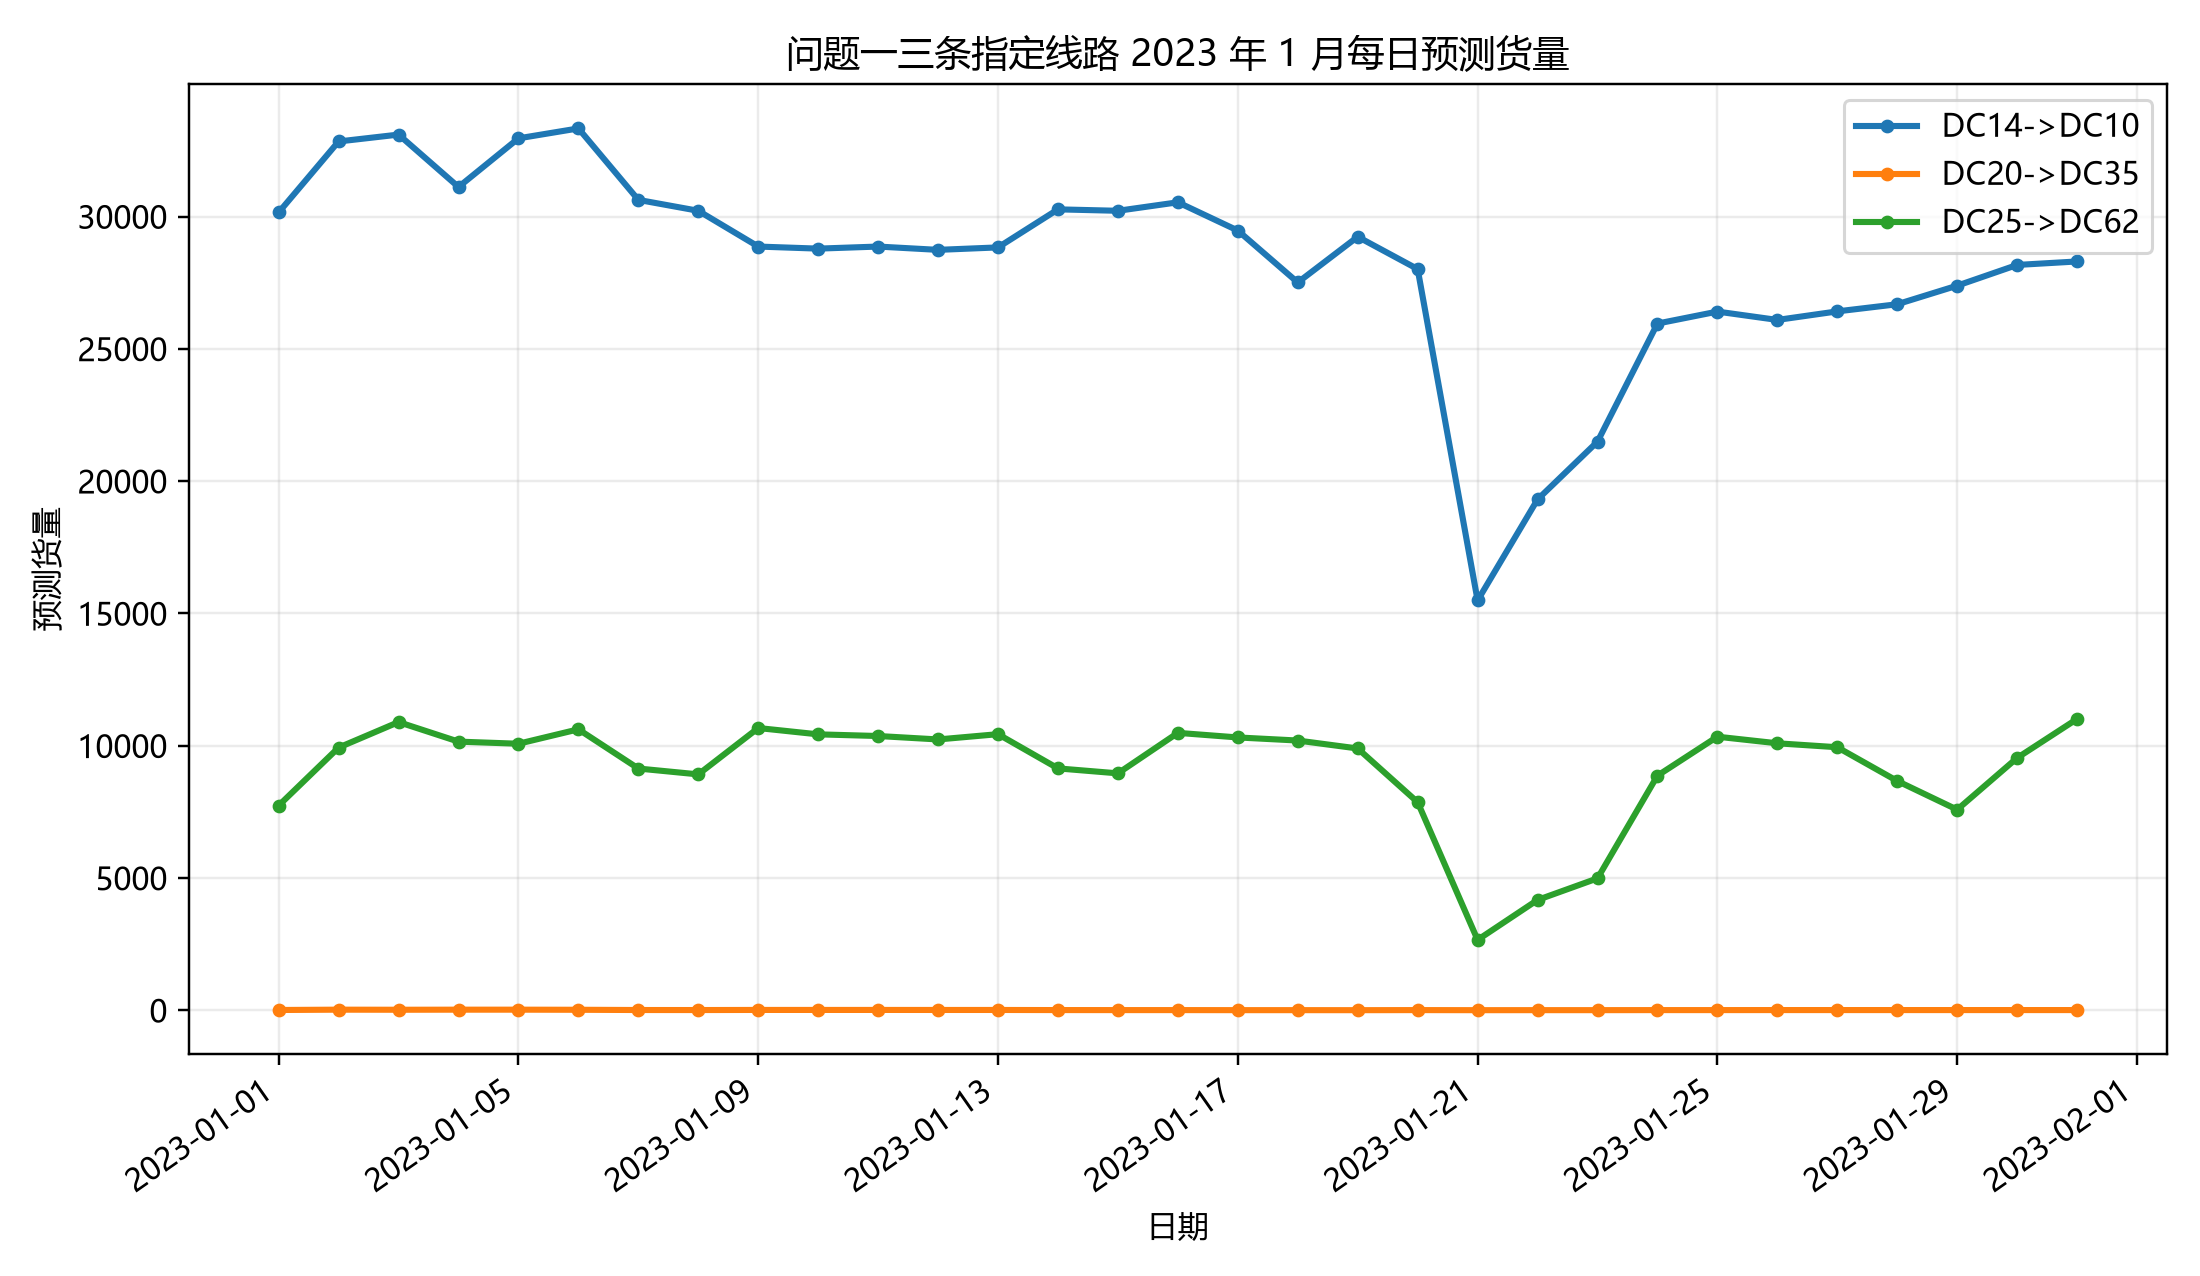
\includegraphics[width=0.86\linewidth]{figures/target_edges.png}
  \caption{三条指定线路 2023 年 1 月每日预测货量}
  \label{fig:target-edges}
\end{figure}

由于 DC20$\rightarrow$DC35 的货量远小于另外两条线路，在三线路对比图中变化不够明显，故单独绘制该线路的每日预测曲线，如图 \ref{fig:dc20-dc35} 所示。可以看出，该线路预测货量整体处于个位数到二十余件之间，春节前后没有明显高峰，符合其低货量稀疏线路的特征。

\begin{figure}[H]
  \centering
  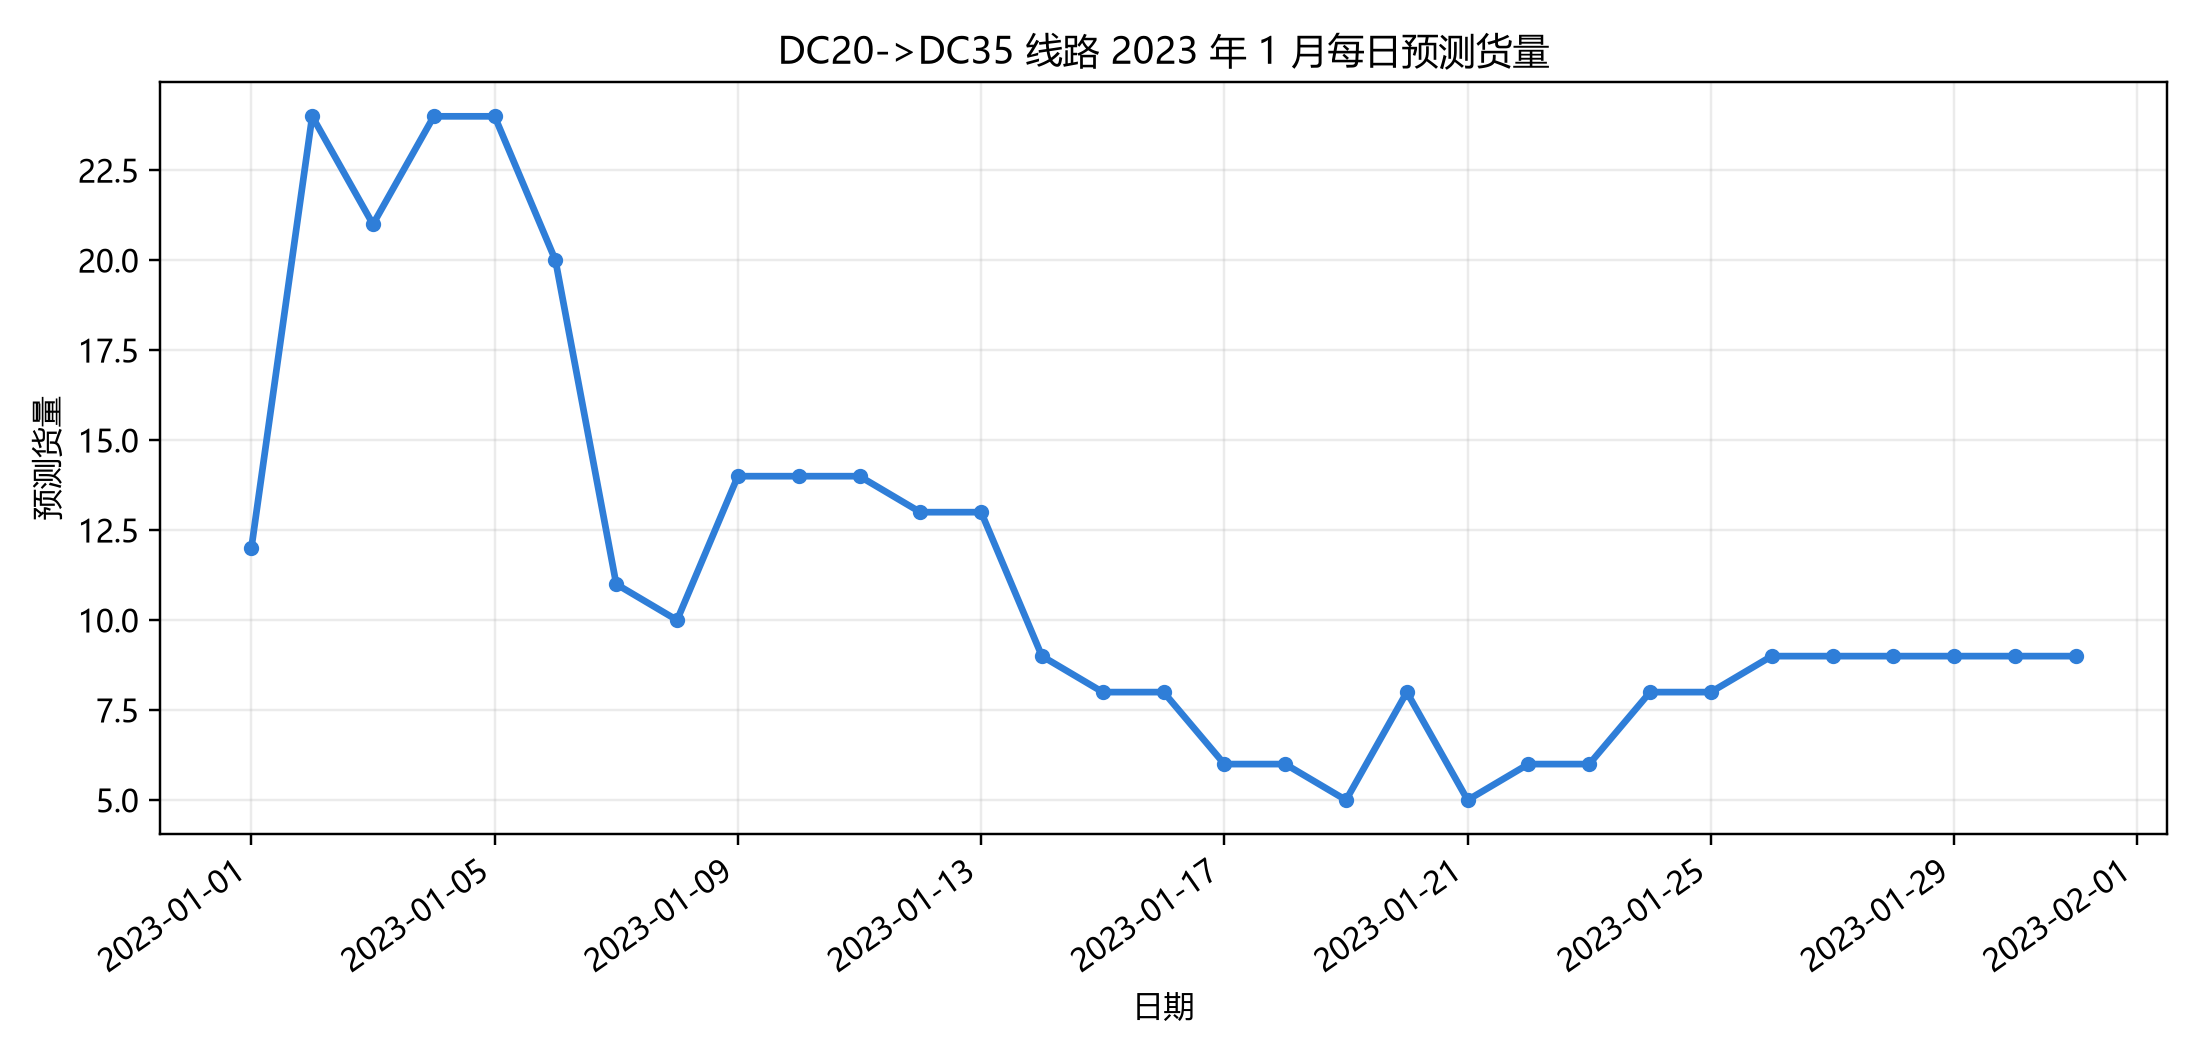
\includegraphics[width=0.82\linewidth]{figures/dc20_dc35_daily.png}
  \caption{DC20$\rightarrow$DC35 线路 2023 年 1 月每日预测货量}
  \label{fig:dc20-dc35}
\end{figure}

表 \ref{tab:target-sum} 给出了三条指定线路的 1 月预测总量。可以看出，DC14$\rightarrow$DC10 的月预测总量为 875410，属于高货量线路；DC20$\rightarrow$DC35 的月预测总量仅为 351，表明该线路在模型判断中仍为小货量线路；DC25$\rightarrow$DC62 的月预测总量为 284330，与 2022 年 1 月和 12 月水平接近。

\begin{table}[H]
  \centering
  \caption{三条指定线路 2023 年 1 月预测总量}
  \label{tab:target-sum}
  \begin{tabular}{lrrr}
    \toprule
    线路 & 2023 年 1 月预测总量 & 2022 年 1 月真实总量 & 2022 年 12 月真实总量 \\
    \midrule
    DC14$\rightarrow$DC10 & 875410 & 1651283 & 828194 \\
    DC20$\rightarrow$DC35 & 351 & 1604 & 1618 \\
    DC25$\rightarrow$DC62 & 284330 & 271938 & 275367 \\
    \bottomrule
  \end{tabular}
\end{table}

三条指定线路的逐日预测结果见表 \ref{tab:target-daily}。该表是题目要求在论文中给出的核心结果之一，完整全线路预测结果另存为 CSV 文件，可作为后续问题二和问题三中线路能力、调运分配和网络负荷计算的输入。

\begin{longtable}{rrrr}
  \caption{三条指定线路 2023 年 1 月每日预测货量}
  \label{tab:target-daily}\\
  \toprule
  日期 & DC14$\rightarrow$DC10 & DC20$\rightarrow$DC35 & DC25$\rightarrow$DC62 \\
  \midrule
  \endfirsthead
  \toprule
  日期 & DC14$\rightarrow$DC10 & DC20$\rightarrow$DC35 & DC25$\rightarrow$DC62 \\
  \midrule
  \endhead
  01-01 & 30157 & 12 & 7739 \\
  01-02 & 32838 & 24 & 9930 \\
  01-03 & 33098 & 21 & 10894 \\
  01-04 & 31117 & 24 & 10155 \\
  01-05 & 32956 & 24 & 10075 \\
  01-06 & 33331 & 20 & 10620 \\
  01-07 & 30630 & 11 & 9138 \\
  01-08 & 30218 & 10 & 8917 \\
  01-09 & 28866 & 14 & 10669 \\
  01-10 & 28788 & 14 & 10430 \\
  01-11 & 28866 & 14 & 10367 \\
  01-12 & 28741 & 13 & 10237 \\
  01-13 & 28834 & 13 & 10437 \\
  01-14 & 30272 & 9 & 9143 \\
  01-15 & 30218 & 8 & 8956 \\
  01-16 & 30539 & 8 & 10486 \\
  01-17 & 29471 & 6 & 10313 \\
  01-18 & 27509 & 6 & 10196 \\
  01-19 & 29236 & 5 & 9896 \\
  01-20 & 28015 & 8 & 7865 \\
  01-21 & 15489 & 5 & 2662 \\
  01-22 & 19308 & 6 & 4171 \\
  01-23 & 21492 & 6 & 4987 \\
  01-24 & 25956 & 8 & 8869 \\
  01-25 & 26408 & 8 & 10341 \\
  01-26 & 26093 & 9 & 10092 \\
  01-27 & 26416 & 9 & 9943 \\
  01-28 & 26686 & 9 & 8668 \\
  01-29 & 27388 & 9 & 7584 \\
  01-30 & 28171 & 9 & 9539 \\
  01-31 & 28303 & 9 & 11011 \\
  \bottomrule
\end{longtable}

\section{本问结论}

问题一建立了基于完整线路--日期面板的全局 LightGBM 货量预测模型。模型将线路类别、日期周期、春节相对日期、滞后货量、滚动统计量和历史静态统计量统一纳入特征向量，在对数货量空间中训练加性回归树模型，并用递推方式完成 2023 年 1 月逐日预测。回测结果表明，该模型相较于基准模型显著降低了线路级预测误差。

针对模型总量偏保守的问题，本文进一步引入春节相对窗口总量校准，将 2023 年 1 月全网预测总量调整为 40086040。最终结果包含全网 1049 条线路 31 天的预测货量，并给出三条指定线路的逐日预测结果。该结果满足非负性、整数性和历史能力检查要求，可作为后续场地关停情形下物流网络应急调运与结构优化的基础输入。

\section{模型评价}

本模型的主要优点在于：第一，采用全局模型同时学习所有线路，缓解了稀疏线路单独建模时样本不足的问题；第二，引入春节相对日期特征，适应 2023 年春节公历日期错位带来的影响；第三，利用滞后和滚动统计特征刻画线路近期状态，使预测结果能反映短期趋势；第四，通过春节窗口总量校准，避免了线路级模型误差在全网总量上的累积偏差。

模型的不足主要在于：历史数据只有两年，春节、大促等特殊事件样本较少，模型对极端峰值的学习仍受限制；DC20$\rightarrow$DC35 等低货量线路预测值偏保守，说明稀疏小线路仍存在一定不确定性；递推预测会使前序预测误差影响后续日期。若进一步改进，可引入更多年份历史数据，或对低货量稀疏线路建立专门的概率校正模型。

\begin{thebibliography}{99}
  \bibitem{lightgbm} Ke G, Meng Q, Finley T, et al. LightGBM: A Highly Efficient Gradient Boosting Decision Tree[C]. Advances in Neural Information Processing Systems, 2017.
  \bibitem{ai-tool} OpenAI Codex, GPT-5, used for modeling discussion, code assistance, result organization and paper drafting, 2026-07-20.
\end{thebibliography}

\CumcmMainMatterEnd
\appendix
\ctexset{section={name={附录,、},number=\Alph{section}}}

\section{支撑材料索引}

\begin{longtable}{L{0.34\textwidth}L{0.16\textwidth}L{0.38\textwidth}}
  \caption{问题一支撑材料文件清单}\label{tab:support-files}\\
  \toprule
  文件名 & 对应内容 & 用途说明 \\
  \midrule
  \endfirsthead
  \toprule
  文件名 & 对应内容 & 用途说明 \\
  \midrule
  \endhead
  \supportfile{problem1_lightgbm_forecast.py}{问题一}{训练普通 LightGBM 模型并输出 2023 年 1 月初始预测结果}
  \supportfile{problem1_final_forecast.py}{问题一}{根据春节相对窗口对 LightGBM 结果进行总量校准并生成最终预测表}
  \supportfile{problem1_final_2023_01_forecast_all_edges.csv}{问题一}{保存 1049 条线路 31 天的最终预测结果}
  \supportfile{problem1_final_2023_01_forecast_target_edges.csv}{问题一}{保存三条指定线路的最终预测结果}
  \bottomrule
\end{longtable}

\section{主要程序代码}

\subsection{LightGBM 预测程序}
\lstinputlisting[language=Python]{code/problem1_lightgbm_forecast.py}

\subsection{最终总量校准程序}
\lstinputlisting[language=Python]{code/problem1_final_forecast.py}

\end{document}
